In this chapter, we consider spinless bosons that have a permanent dipole moment and are trapped in an optical lattice. Since dipole-dipole interactions fall off as $V(r) \sim 1/r^3$, the contact interaction alone results in a poor description of the system. To remedy this, we take into account the nearest neighbour interactions as well.
\begin{equation}
    H = -t\sum_{\langle i, j\rangle} a_i^{\dagger}a_j + \frac{U}{2}\sum_i n_i(n_i - 1) + \frac{V}{2}\sum_{\langle i, j \rangle} n_i n_j - \mu \sum_i n_i
\end{equation}
Such a Hamiltonian is generally called the Extended Bose-Hubbard model (eBHM)\cite{Baier16}. The analysis that follows will apply for any microscopic interactions that are long-range in nature to justify considering the nearest neighbour interactions, and not just those that have a dipolar origin. The details only become relevant if we wish to compute experimentally achievable values of $V$\cite{Zhang_2021} (as in Sec. \ref{sec:calc_params}). However, we will not be dealing with this in the thesis.
\vspace{0.5cm}\\
We are specifically interested in the case when $U, V > 0$. In such a situation, the on-site and nearest neighbour interactions compete with each other, introducing the possibility of breaking the translational symmetry. We proceed now to study how this affects the ground-state phases through a mean-field analysis. 

\section{Mean Field Theory}
The mean-field decoupling of the eBHM largely proceeds the same way as with the BHM. The key difference is that we also need to decouple the $n_in_j$ term by introducing another set of mean-field parameters, $\{\rho_i\}$. 

\begin{minipage}{0.5\linewidth}
    \begin{align}
        &\hspace{1.2cm}\hat{a}_i = \Psi_i + \delta \hat{a}_i \nonumber\\
        &\implies \delta a_i^{\dagger} \delta a_j = (a_i^{\dagger} - \Psi_i^*)(a_j - \Psi_j) \approx 0 \nonumber\\
        &\implies a_i^{\dagger}a_j \approx \Psi_ja_i^{\dagger} + \Psi_i^*a_j - \Psi_i^*\Psi_j \nonumber
    \end{align}
\end{minipage}%
\begin{minipage}{0.5\linewidth}
    \begin{align}
        &\hspace{1.2cm}\hat{n}_i = \rho_i + \delta \hat{n}_i \nonumber\\
        &\implies \delta n_i \delta n_j = (n_i - \rho_i)(n_j - \rho_j) \approx 0 \nonumber\\
        &\implies n_i n_j \approx \rho_j n_i + \rho_i n_j - \rho_i\rho_j
    \end{align}
\end{minipage}
\vspace{0.5cm}\\
Note here that since $n_i = a_i^{\dagger}a_i$, we could have simply used the first decoupling for the $n_i n_j$ term as well. However, the resulting mean-field Hamiltonian turns out to be incapable of hosting the phases we are interested in. In any case, neglecting the terms of $\mathcal{O}(\delta a_i^2)$ is a lower order approximation than neglecting $\mathcal{O}(\delta n_i^2)$.
\vspace{0.5cm}\\
Proceeding with the derivation, we already know the decoupling for the hopping term from Eq. \eqref{eq:mft_hop}. The decoupling for the interaction term proceeds in a similar way. 
\begin{align}
    H_{int}/(V/2) &= \sum_{\langle i, j\rangle} n_i n_j \nonumber\\
    &= \sum_{\langle i, j\rangle} (\rho_jn_i + \rho_in_j - \rho_i\rho_j) \nonumber\\
    &= \sum_i \big (\sum_{j \in N_i} \rho_j\big ) n_i + \sum_i \big (\sum_{j \in N_i} \rho_j\big ) n_i - \sum_i \big (\sum_{j \in N_i} \rho_j\big) \rho_i
\end{align}

Defining the mean order parameter, $\overline{\rho}_i = \frac{1}{z}\sum_{j \in N_i} \rho_j$, we obtain the interaction term at the mean-field level.
\begin{align}
    H_{int}/(zV/2) = \sum_i (2\overline{\rho}_i n_i - \overline{\rho}_i\rho_i)
\end{align}
We can then write the entire site-decoupled Hamiltonian which depends on a set of $2M$
mean-field parameters, $\{\Psi_i, \rho_i\}$.
\begin{equation}
    H_i\{\Psi_i, \rho_i\} = -zt (\overline{\Psi}_i a_i^{\dagger} + \overline{\Psi}_i^* a_i - \overline{\Psi}_i\Psi_i^*) + \frac{zV}{2} (2\overline{\rho}_i n_i - \overline{\rho}_i\rho_i) + \frac{U}{2}n_i(n_i - 1) - \mu n_i
\end{equation}

Following the derivation in Sec. \ref{sec:bhm_mft}, we might now be tempted to set $\Psi_i = \Psi \text{ and } \rho_i = \rho$. However, this is a bad choice to make for the eBHM, because as mentioned earlier, the interplay of the interaction terms allows the possibility of breaking the translational symmetry. Making this assumption would incorrectly ignore the existence of certain phases and misrepresent the extents of others. Instead, we can consider arbitrary periodic patterns across the lattice and write the mean-field Hamiltonian for a single unit-cell\cite{Gheeraert2011} as follows.
\begin{align}\label{eq:ebhm_mft}
    H_{MF, UC} = &\sum_{X \in UC} \left [-zt(\overline{\Psi}_X a_X^{\dagger} + \overline{\Psi}_X^* a_X) + (zV\overline{\rho}_X - \mu)n_X + \frac{U}{2}n_X(n_X - 1)\right ] \nonumber\\
    - &\sum_{X \in UC} \left [zt\overline{\Psi}_i\Psi_i^* -  \frac{zV}{2} \overline{\rho}_X\rho_X \right ]
\end{align}


\section{Results}

\subsection{1D lattice}
Since the interaction term only acts between nearest neighbour pairs, there is only one periodic pattern that is possible for the 1D lattice. This simply comprises of a unit cell with two sites $A$ and $B$ that repeat through the lattice. It is prudent now to introduce the notion of a connectivity matrix that uniquely specifies the unit cell.

\begin{minipage}{0.4\linewidth}
    \begin{equation*}
        M_{UC} =  \bordermatrix{ & A & B \cr
        A & 0 & 2 \cr
        B & 2 & 0 }
    \end{equation*}
\end{minipage}%
\begin{minipage}{0.5\linewidth}
%%% FIG %%%
\centering
\vspace{0.2cm}
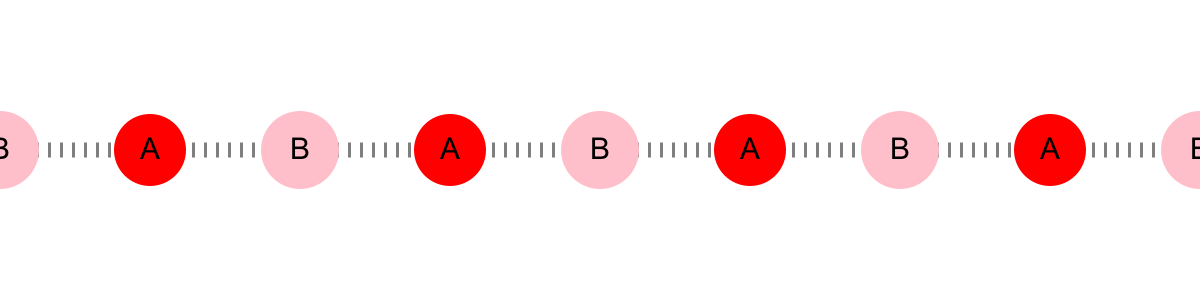
\includegraphics[width = 0.8\textwidth]{ch5/1d_sublattice.png}
%%% FIG %%%
\end{minipage}
\vspace{0.5cm}\\
Such a matrix is always symmetric and is equivalent to representing the lattice as an undirected graph. Although this is not strictly required for the 1D chain, we will find it useful to distinguish different patterns in more complicated lattice geometries. The connectivity matrix also gives us a succinct way to compute the mean-field parameters.
\begin{equation}\label{eq:unit_cell}
    \begin{pmatrix}
        \overline{\Psi}_A \\
        \overline{\Psi}_B
    \end{pmatrix} = M_{UC}  \begin{pmatrix}
        \Psi_A \\
        \Psi_B
    \end{pmatrix}
\end{equation}
which in this case simply gives us $\overline{\Psi}_A = 2\Psi_B$ and $\overline{\Psi}_B = 2\Psi_A$. The same relation also holds for $\overline{\rho}_X$ and $\rho_X$. We can now construct the Hamiltonian and self-consistently diagonalize it to obtain the ground state solution.

\subsubsection{\large Classifying the phases}
Note that we now have four mean-field parameters, $\{\Psi_A, \Psi_B, \rho_A, \rho_B\}$ and the various phases can be classified using them as follows.
\begin{itemize}
    \item When $\rho_A = \rho_B = \rho$ and $\Psi_A = \Psi_B = \Psi$, this effectively restores translational invariance and describes a Mott Insulator when $\Psi = 0$ and a Superfluid otherwise.
\end{itemize}
%%% FIG %%%
\begin{figure}[!htb]
    \centering
    \begin{subfigure}[b]{0.45\textwidth}  %keep total sum <1 to show in same line
        \centering
        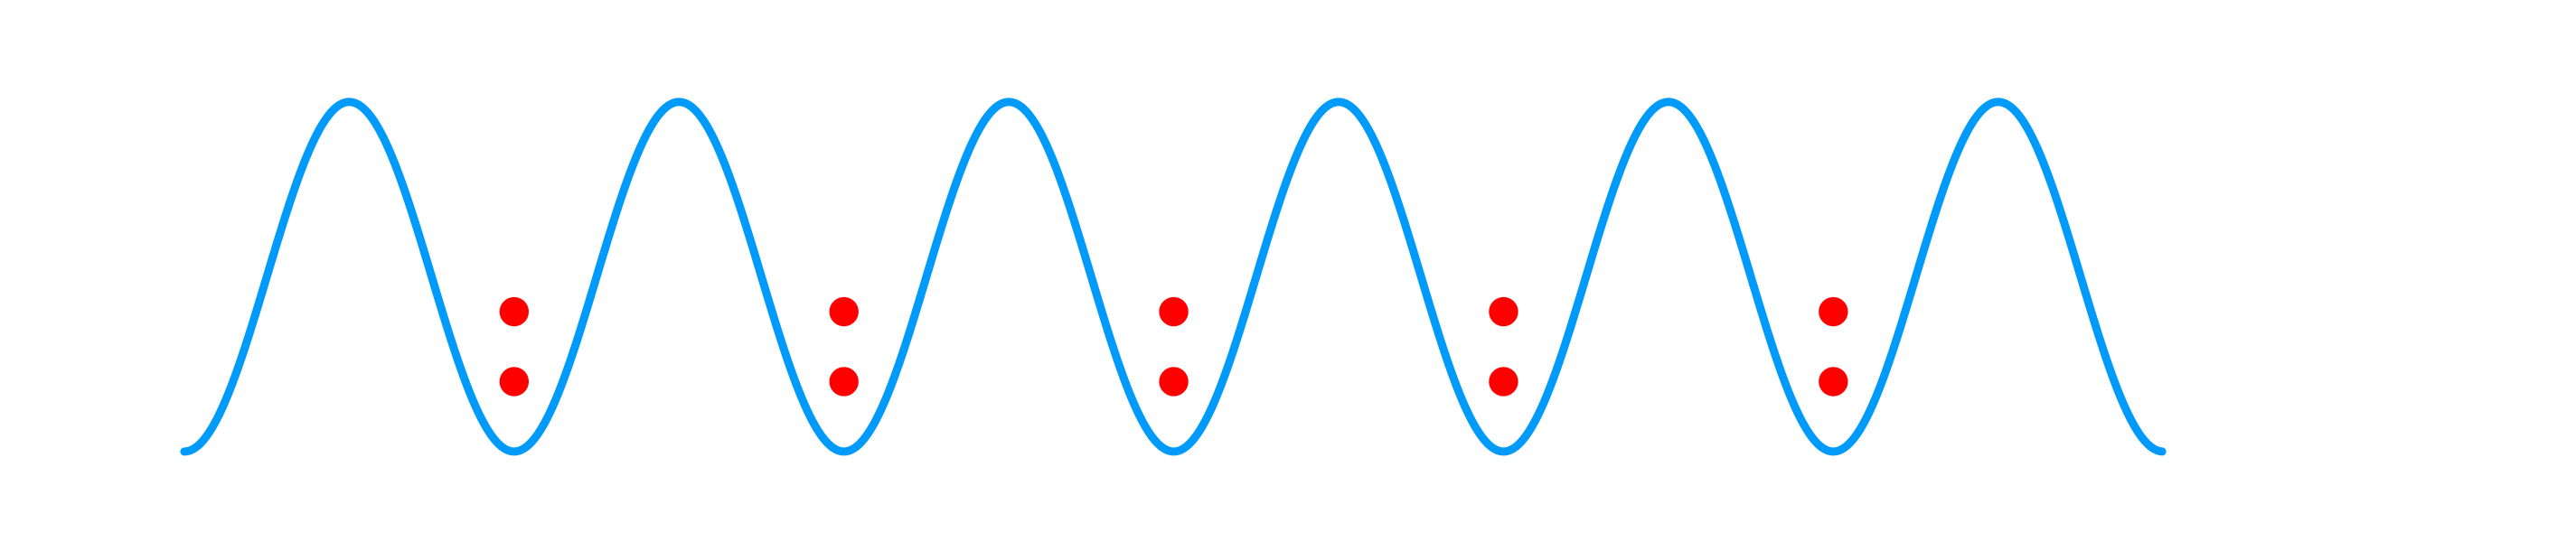
\includegraphics[width=\textwidth]{ch5/MIdiagram.png}
        \caption{Mott insulator}
    \end{subfigure}
    \hspace{1em}  %\hfill
    \begin{subfigure}[b]{0.45\textwidth}
        \centering
        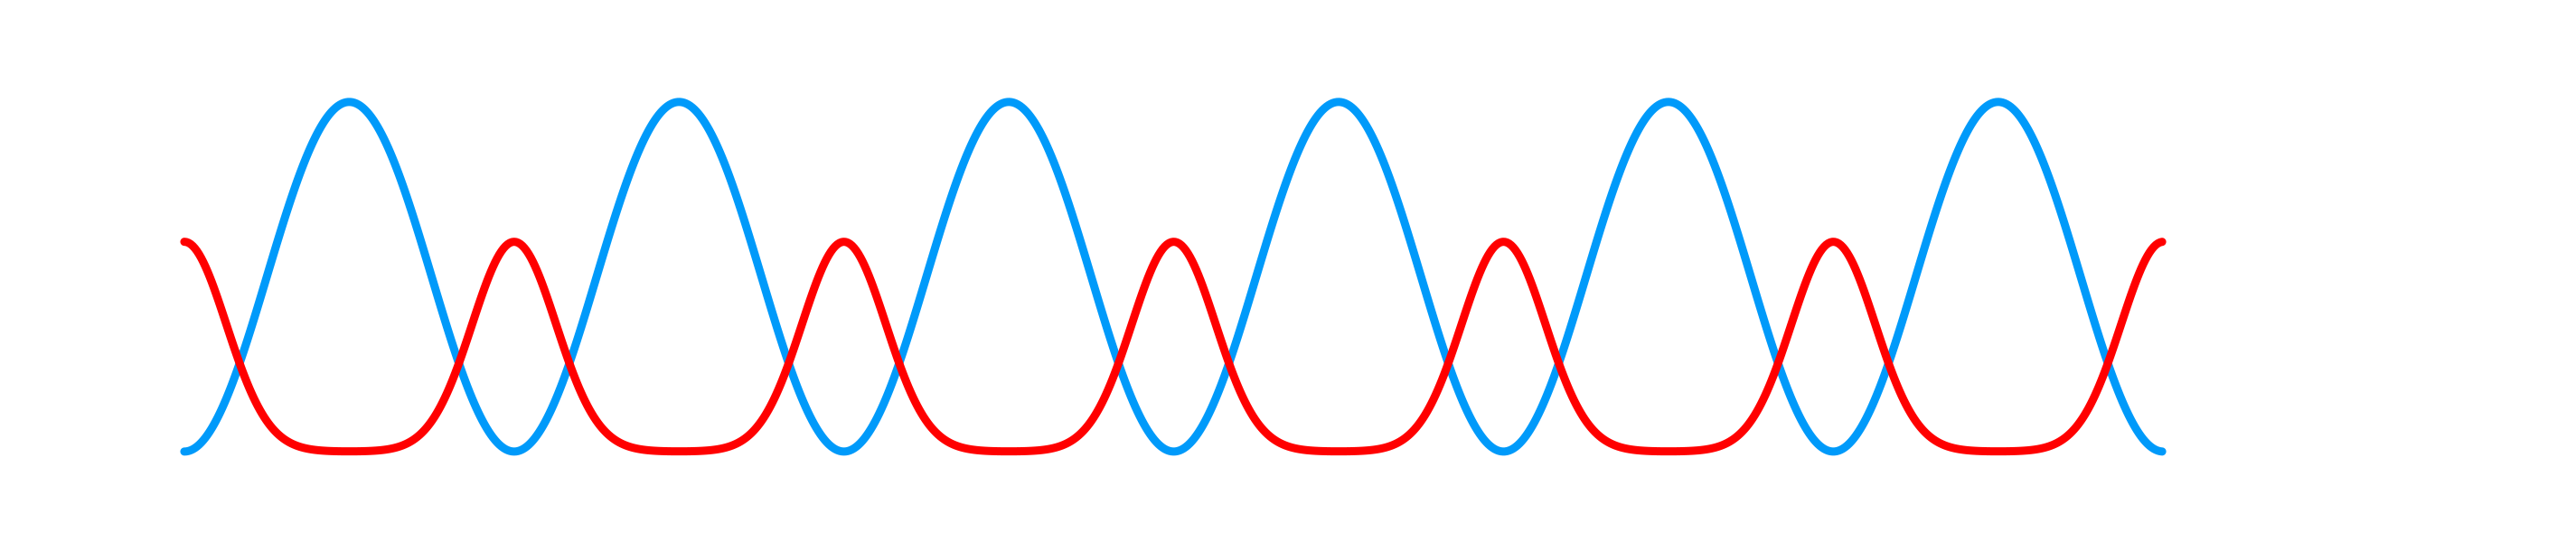
\includegraphics[width=\textwidth]{ch5/SFdiagram.png}
        \caption{Super-fluid}
    \end{subfigure}
    \caption{Pictorial representation of the BHM phases}
    \label{}
\end{figure}
%%% FIG %%%
\FloatBarrier \!\!\!\!\!\!\!\!\!\!\!
\vspace{-0.3cm}
\begin{itemize}
    \item When $\rho_A \neq \rho_B$, this indicates a modulation of the average density of particles over the lattice and describes a Density Wave when $\Psi_A = \Psi_B = 0$ and a Supersolid otherwise.
\end{itemize}

%%% FIG %%%
\begin{figure}[!htb]
    \centering
    \begin{subfigure}[b]{0.45\textwidth}  %keep total sum <1 to show in same line
        \centering
        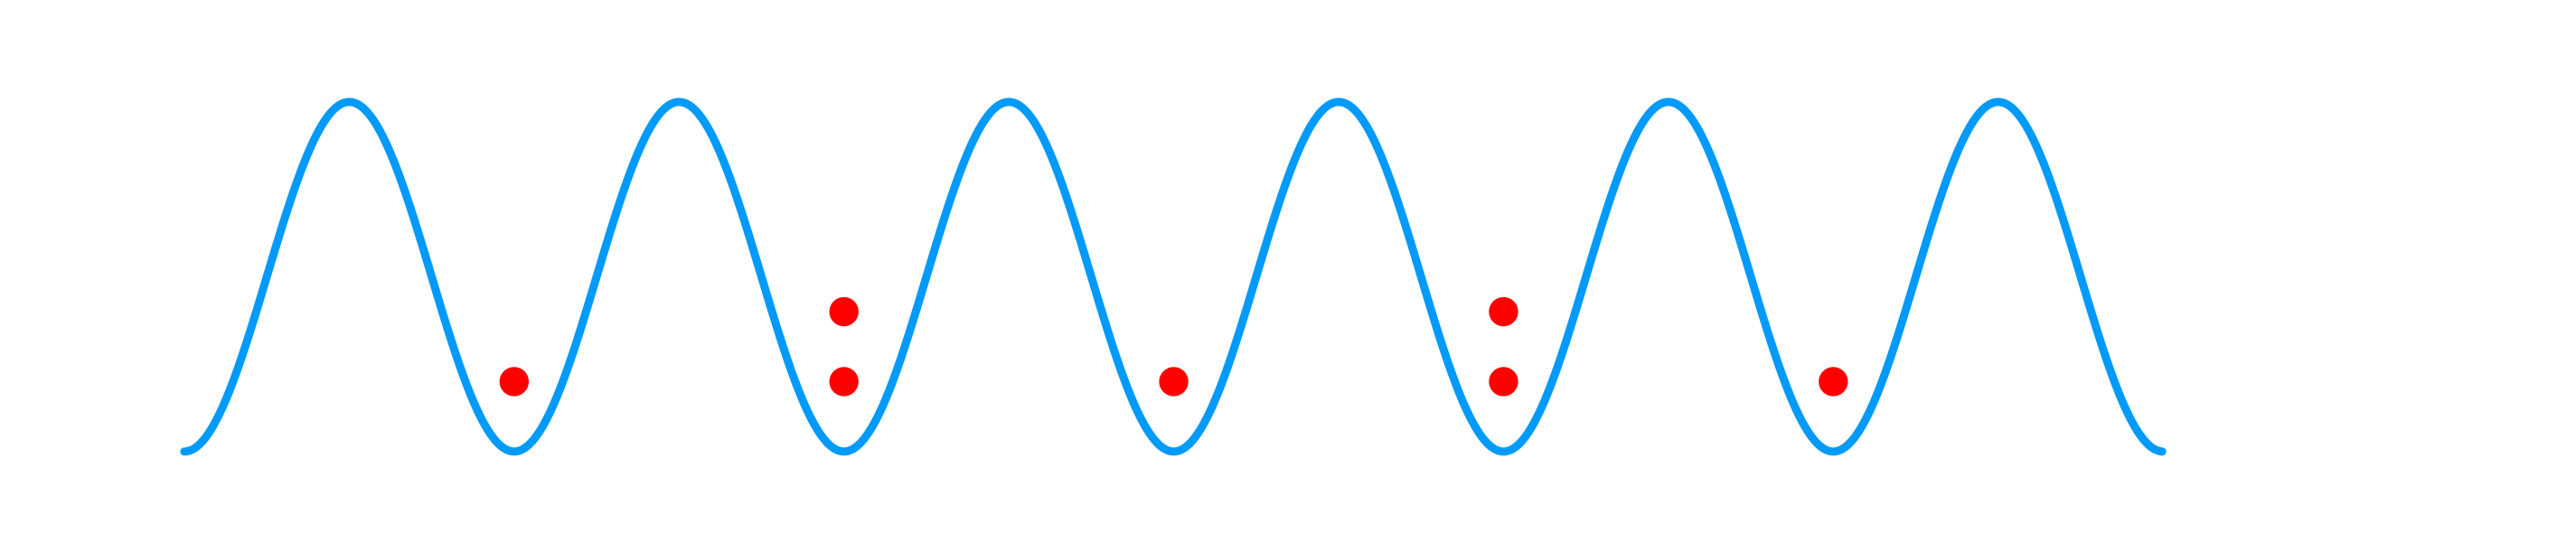
\includegraphics[width=\textwidth]{ch5/DWdiagram.png}
        \caption{Density Wave}
    \end{subfigure}
    \hspace{1em}  %\hfill
    \begin{subfigure}[b]{0.45\textwidth}
        \centering
        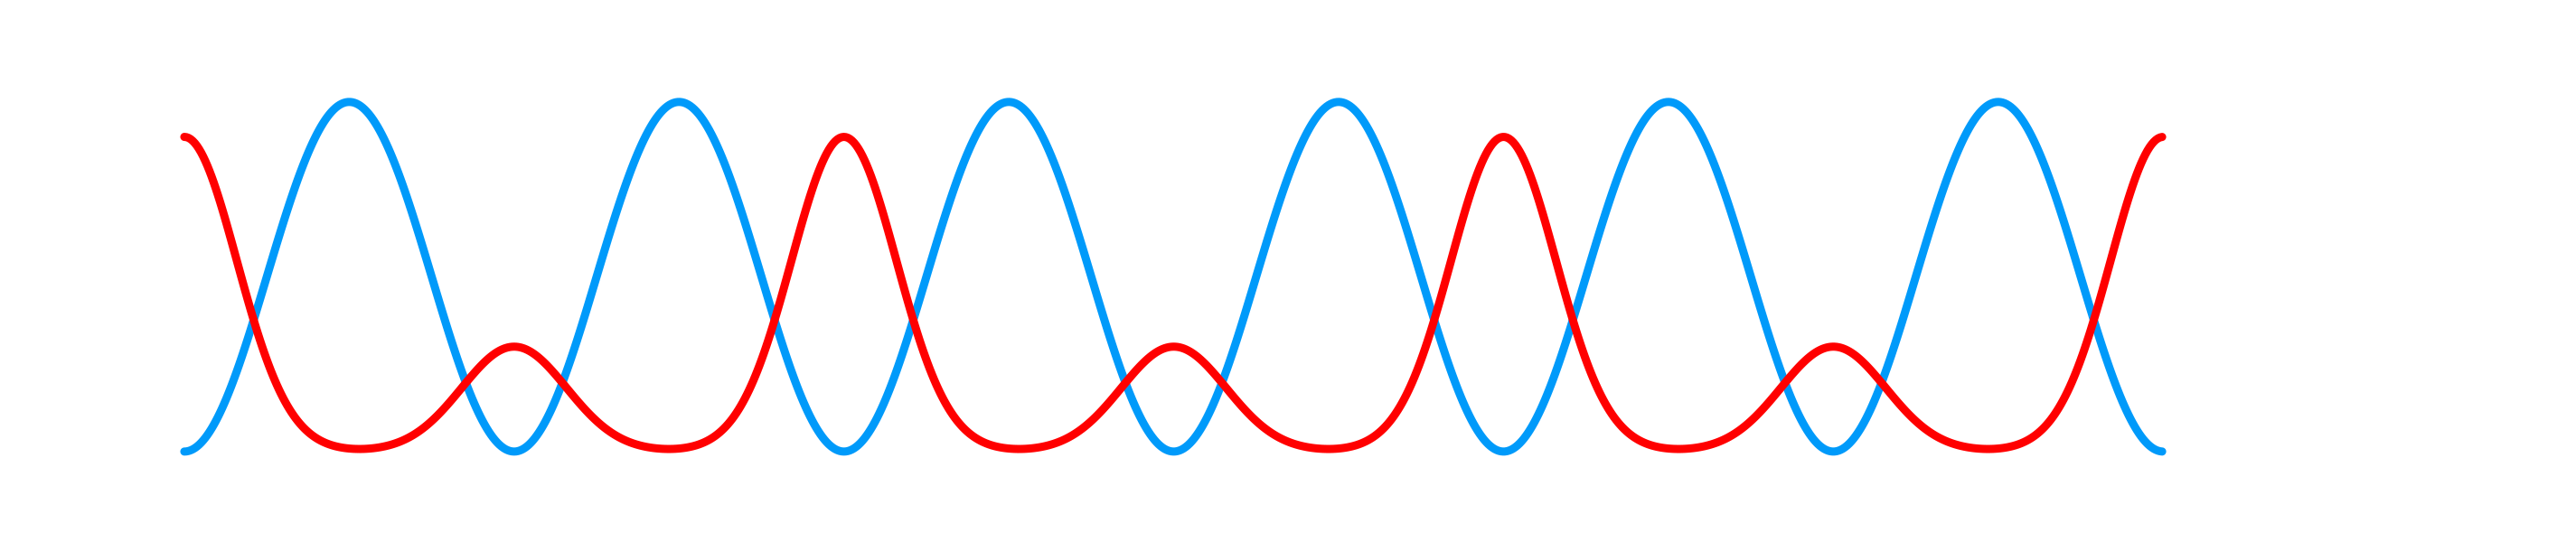
\includegraphics[width=\textwidth]{ch5/SSdiagram.png}
        \caption{Super-solid}
    \end{subfigure}
    \caption{Pictorial representation of the eBHM phases}
    \label{}
\end{figure}
%%% FIG %%%
\FloatBarrier \!\!\!\!\!\!\!\!\!\!\!

It is not surprising that the eBHM also hosts Mott insulator and superfluid phases since the BHM can be recovered in the limit $V\to 0$. When we have $zV \sim U$, however, two new analogous phases are introduced due to density modulations. The density wave phase can simply be interpreted as two inter-weaving Mott insulators with different occupation numbers. On the other hand, the supersolid can naively be described as a phase that exhibits superflow while also having some kind of crystalline order due to the periodic density modulations. Such an interpretation is rather imprecise\cite{Boninsegni_2012}, but the characterization of the phase is unambiguous atleast at the mean-field level.

%%% FIG %%%
\begin{figure}[!htb]
    \centering
    \begin{subfigure}[b]{\textwidth}  %keep total sum <1 to show in same line
        \centering
        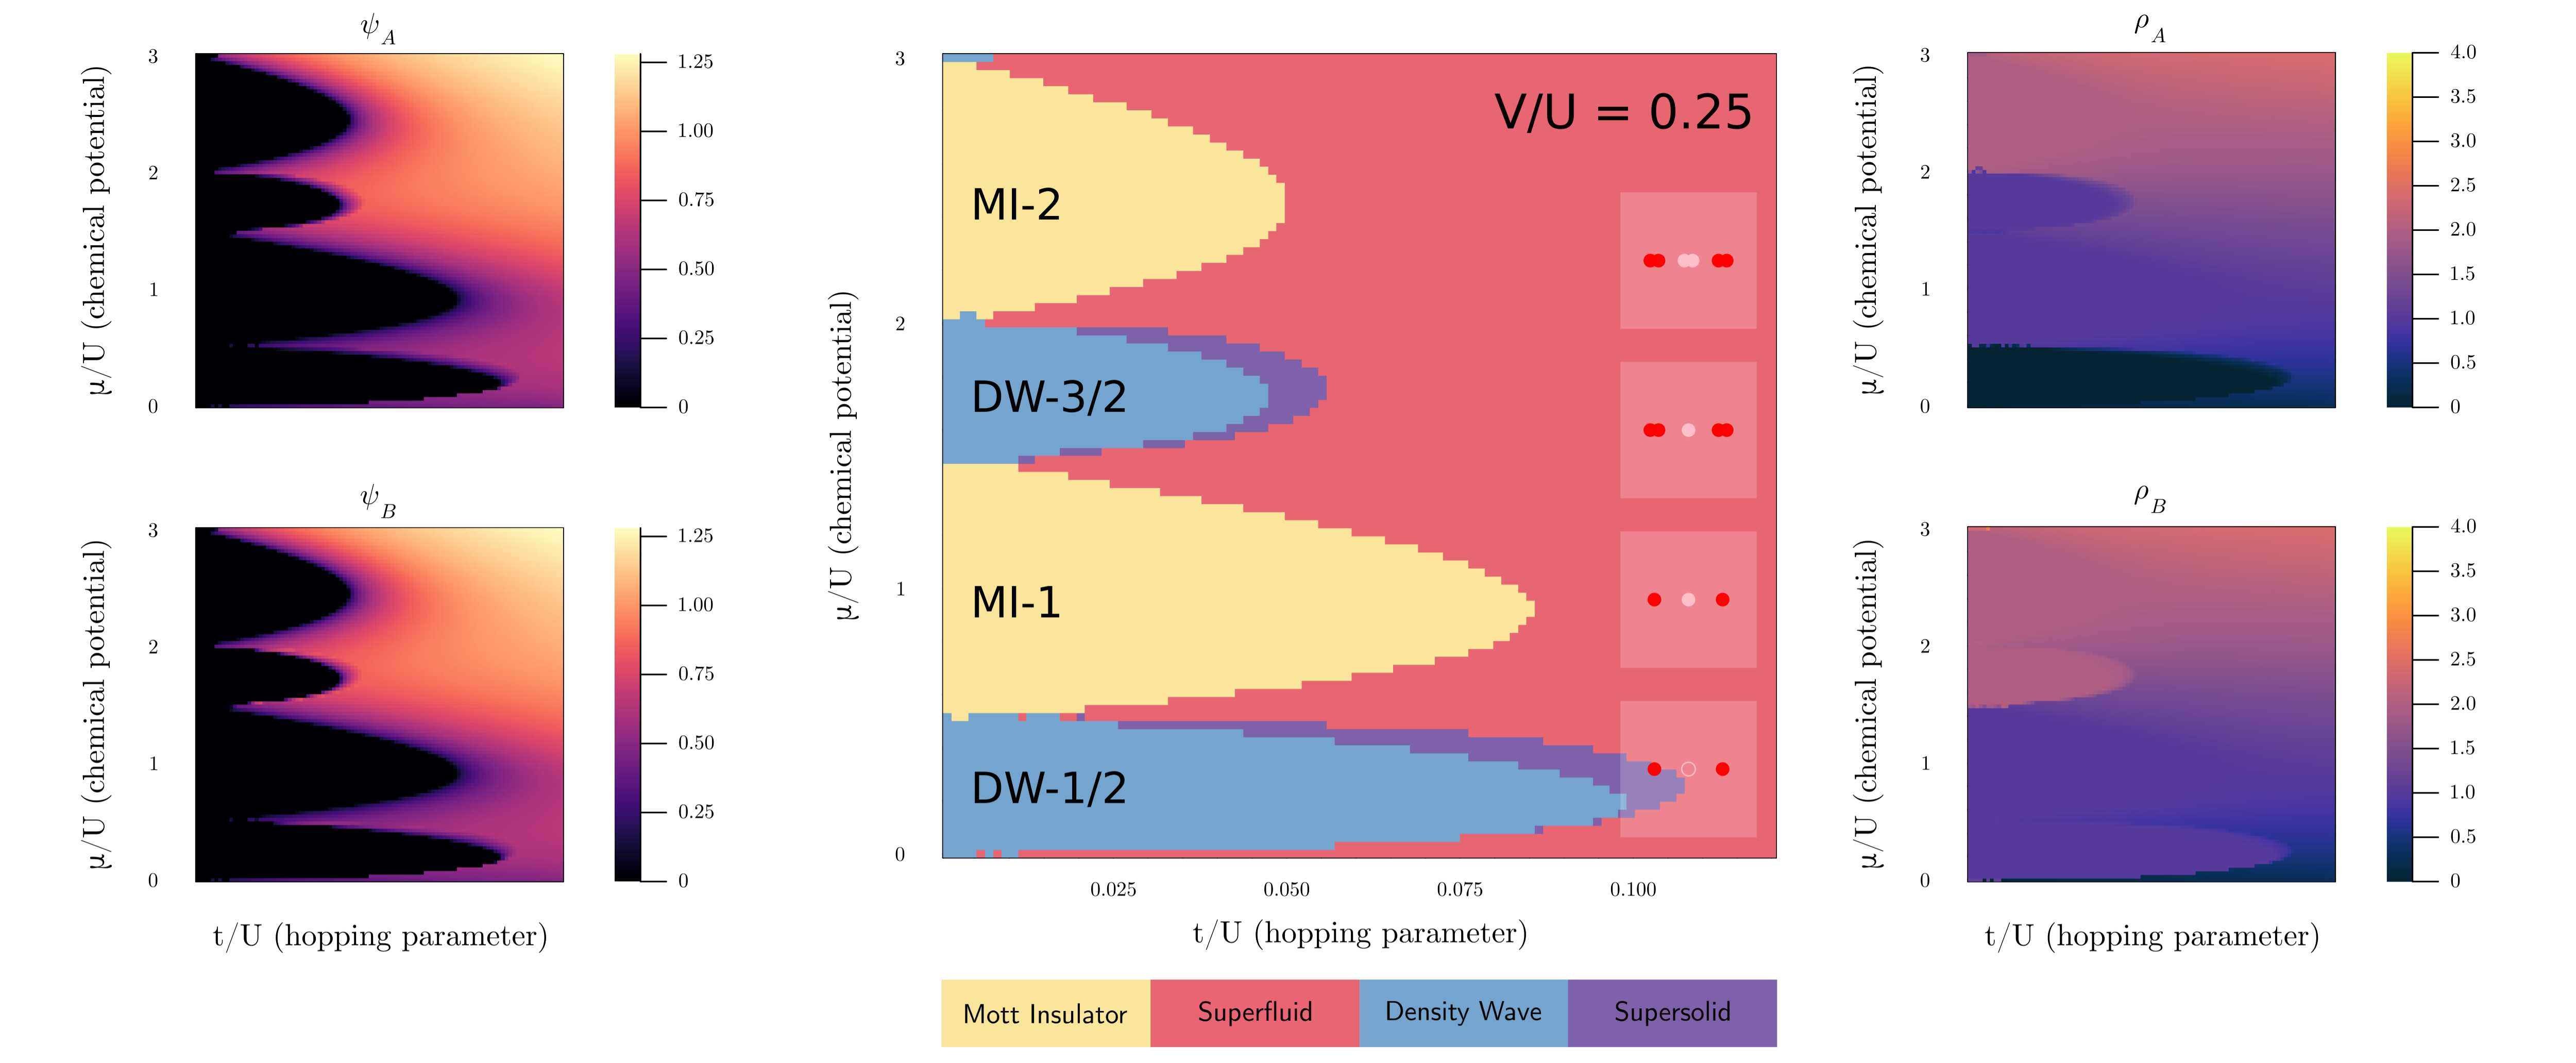
\includegraphics[width=\textwidth]{ch5/1dnew.png}
    \end{subfigure}
    \caption{Mean-field phase diagram of 1D lattice}
    \label{fig:ebhm_1d}
\end{figure}
%%% FIG %%%
\FloatBarrier \!\!\!\!\!\!\!\!\!\!\!

We can see from Fig. \ref{fig:ebhm_1d} that for an intermediate value of $V/U$, all four phases can exist in the $t-\mu$ plane. The density wave seems to appear as lobes in a similar manner to the Mott insulator. Peculiarly, the supersolid phase is only ever observed at the 'edges' of these density wave lobes. Consequently, there is no possibility of finding a phase transition directly from the density wave to the superfluid phase. Similarly, there is no direct transition from a Mott insulator to a supersolid. This seems to support the fact that a quantum phase transition can only occur if it involves breaking a single symmetry of the system.
\vspace{0.5cm}\\
We also note that we can label the density wave lobes with their average filling just as we differentiated Mott insulator lobes with their occupation number. However, this does not uniquely identify them, since a density wave having a filling of $(1, 2)$ and $(0, 3)$ will both have an average occupation of $3/2$ as seen in Fig. \ref{fig:ebhm_sq}.

\newpage
\subsection{2D square lattice}
For a square lattice, we can come up with more than one possible repeating unit cell that breaks translational symmetry. In such a case, we must find the solution in either case and only admit the one having lowest ground state energy.

\begin{minipage}{0.4\linewidth}
    \begin{equation*}
        M_{UC} =  \bordermatrix{ & A & B \cr
        A & 0 & 4 \cr
        B & 4 & 0 }
    \end{equation*}
\end{minipage}%
\hfill
\begin{minipage}{0.5\linewidth}
%%% FIG %%%
\centering
\vspace{0.2cm}
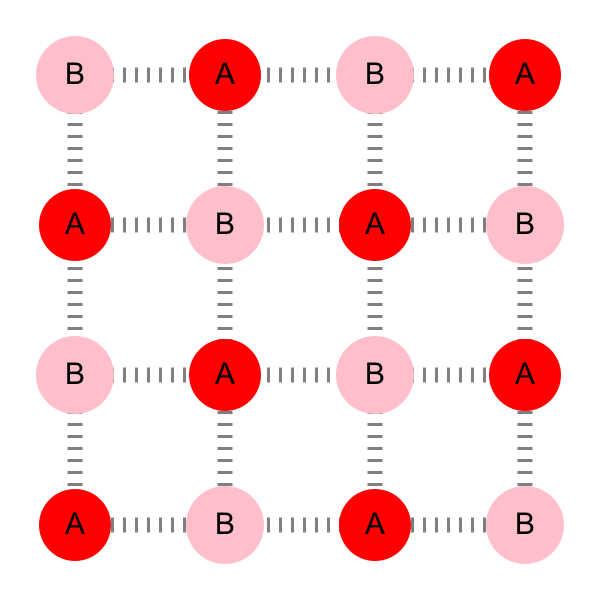
\includegraphics[width = 0.5\textwidth]{ch5/sq_sublattice1.png}
%%% FIG %%%
\end{minipage}
\vspace{0.5cm}\\
\begin{minipage}{0.4\linewidth}
    \begin{equation*}
        M_{UC} =  \bordermatrix{ & A & B \cr
        A & 2 & 2 \cr
        B & 2 & 2 }
    \end{equation*}
\end{minipage}%
\hfill
\begin{minipage}{0.5\linewidth}
%%% FIG %%%
\centering
\vspace{0.2cm}
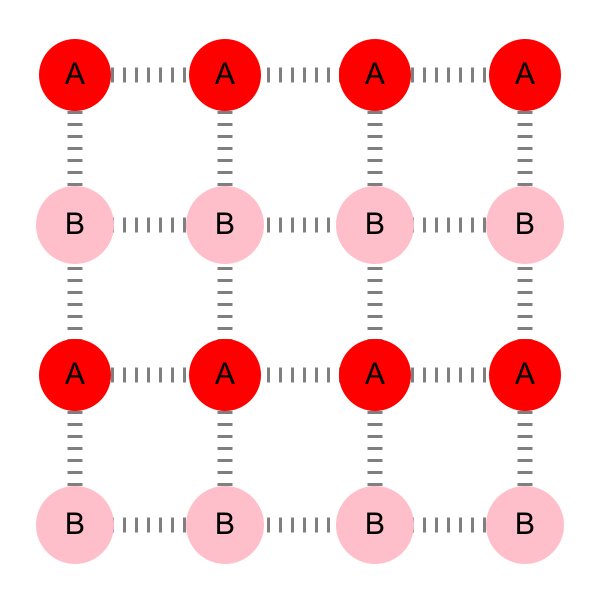
\includegraphics[width = 0.5\textwidth]{ch5/sq_sublattice2.png}
%%% FIG %%%
\end{minipage}
\vspace{0.3cm}\\
It turns out that the first pattern satisfies this condition for all parameter regimes of interest. 
\vspace{-0.4cm}
%%% FIG %%%
\begin{figure}[!htb]
    \centering
    \begin{subfigure}[b]{0.77\textwidth}  %keep total sum <1 to show in same line
        \centering
        \includegraphics[width=\textwidth]{ch5/sq_2dnew.png}
    \end{subfigure}
    \caption{Mean-field phase diagrams of 2D square lattice}
    \label{fig:ebhm_sq}
\end{figure}
%%% FIG %%%
\FloatBarrier \!\!\!\!\!\!\!\!\!\!\!

We see in Fig. \ref{fig:ebhm_sq} that the phase diagram for a 2D square lattice qualitatively looks similar to that of the 1D lattice in Fig. \ref{fig:ebhm_1d}. This is because the connectivity matrix of the dominant pattern in either case is only different by a scaling factor of two. We also see that as $V/U$ is increased, the density wave lobes arise between Mott insulator lobes and increase in extent until the latter becomes unstable throughout the $t-\mu$ plane. Also note that the density waves become the dominant phase in the diagram roughly when $zV \sim U$ as one would expect. As a result, the phase diagram is quite rich since it not only involves transitions between different phases but also between different orders (filling fractions) of density waves.

\subsection{2D triangular lattice}
We consider the following sub-lattice pattern for our analysis of the triangular lattice.

\begin{minipage}{0.4\linewidth}
    \begin{equation*}
        M_{UC} =  \bordermatrix{ & A & B & C \cr
        A & 0 & 3 & 3 \cr
        B & 3 & 0 & 3 \cr
        C & 3 & 3 & 0 }
    \end{equation*}
\end{minipage}%
\hfill
\begin{minipage}{0.5\linewidth}
%%% FIG %%%
\centering
\vspace{0.2cm}
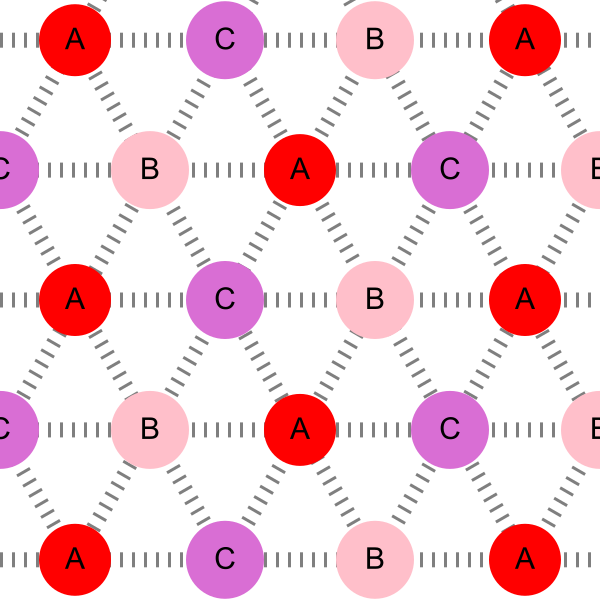
\includegraphics[width = 0.5\textwidth]{ch5/tri_sublattice1.png}
%%% FIG %%%
\end{minipage}
\vspace{0.5cm}\\

We can see in Fig. \ref{fig:ebhm_tri} that the phase diagram is quite similar to that of the square lattice except for one qualitative difference. There are now two density wave lobes between each pair of Mott insulator lobes due to possibility of additional fractional fillings in the triangular lattice (i.e, $1/3$, $2/3$, etc). 

%%% FIG %%%
\begin{figure}[!htb]
    \centering
    \begin{subfigure}[b]{0.81\textwidth}  %keep total sum <1 to show in same line
        \centering
        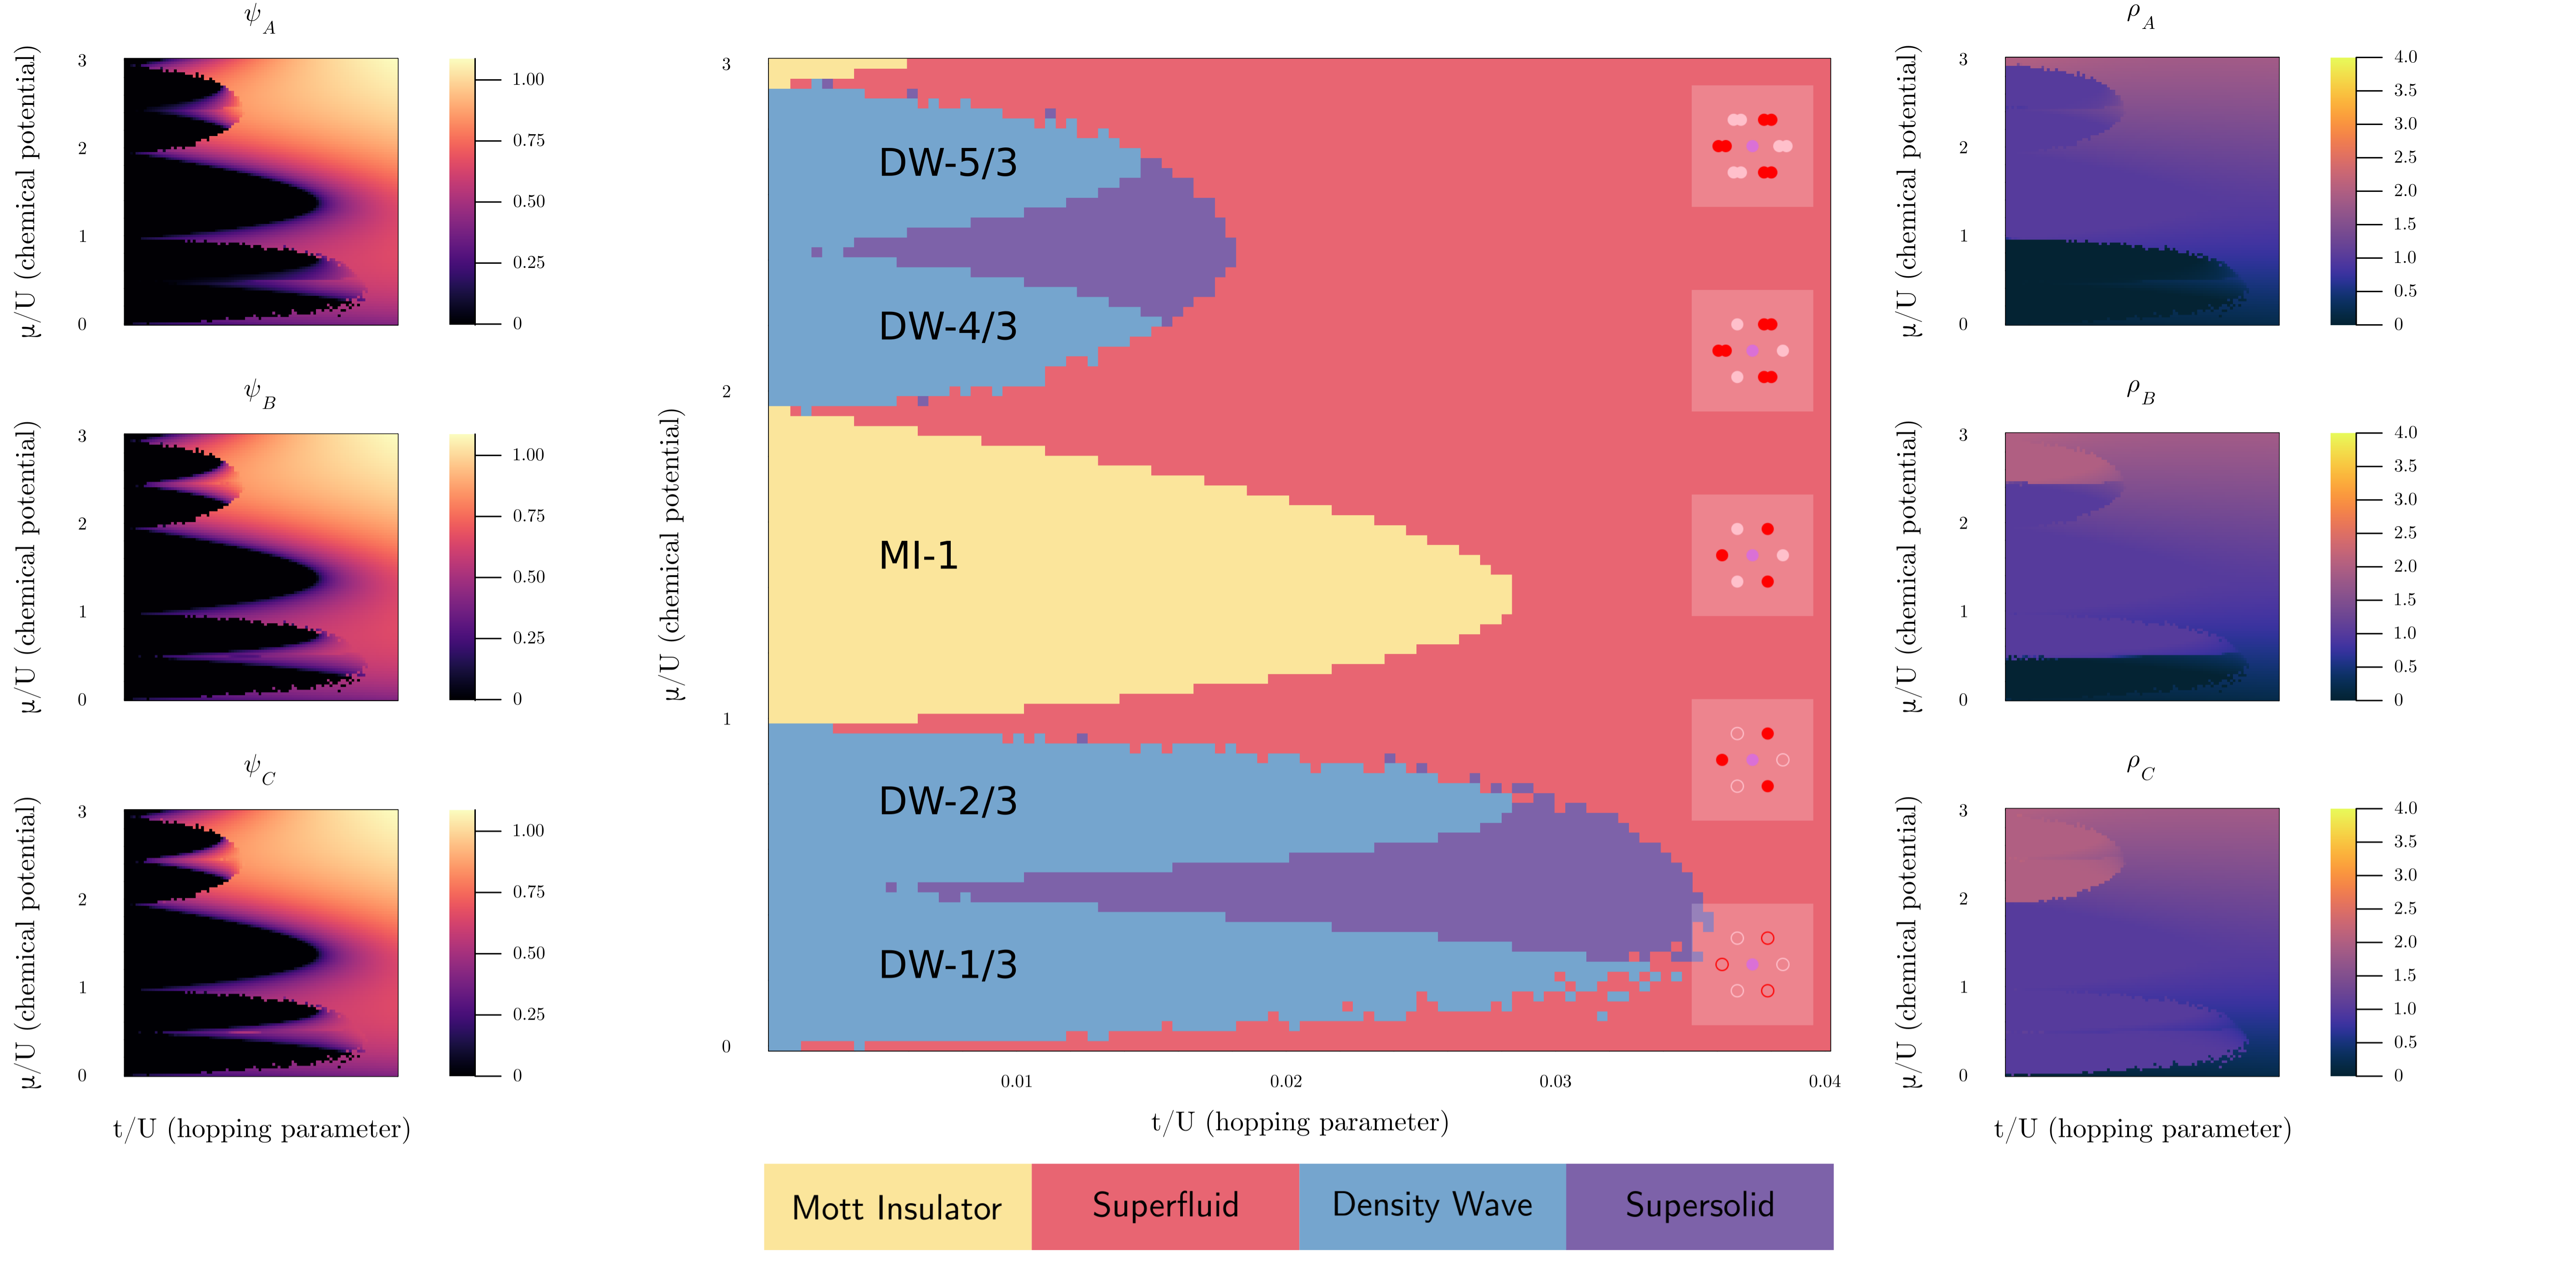
\includegraphics[width=\textwidth]{ch5/tri_2dnew.png}
    \end{subfigure}
    \caption{Mean-field phase diagram of triangular lattice (V/U = 0.34)}
    \label{fig:ebhm_tri}
\end{figure}
%%% FIG %%%
\FloatBarrier \!\!\!\!\!\!\!\!\!\!\!

\section{Issues with self-consistency}\label{sec:caveats}
When we introduced the idea of self-consistency in Chapter 4, we also described the procedure in terms of finding the fixed point of a function. This holds true for the eBHM as well, except the function is now multi-variate which significantly complicates things. For instance, our naive decision to utilize Fixed Point iteration without evaluating the conditions required for convergence has finally caught up with us. 
\vspace{0.5cm}\\
Unfortunately, the order parameters are generally related in a highly non-linear way which makes it hard to determine these conditions analytically. Instead, below are the problems that were encountered while numerically solving the system, along with possible solutions to mitigate them.

%%% FIG %%%
\begin{figure}[!htb]
    \centering
    \begin{subfigure}[b]{0.45\textwidth}  %keep total sum <1 to show in same line
        \centering
        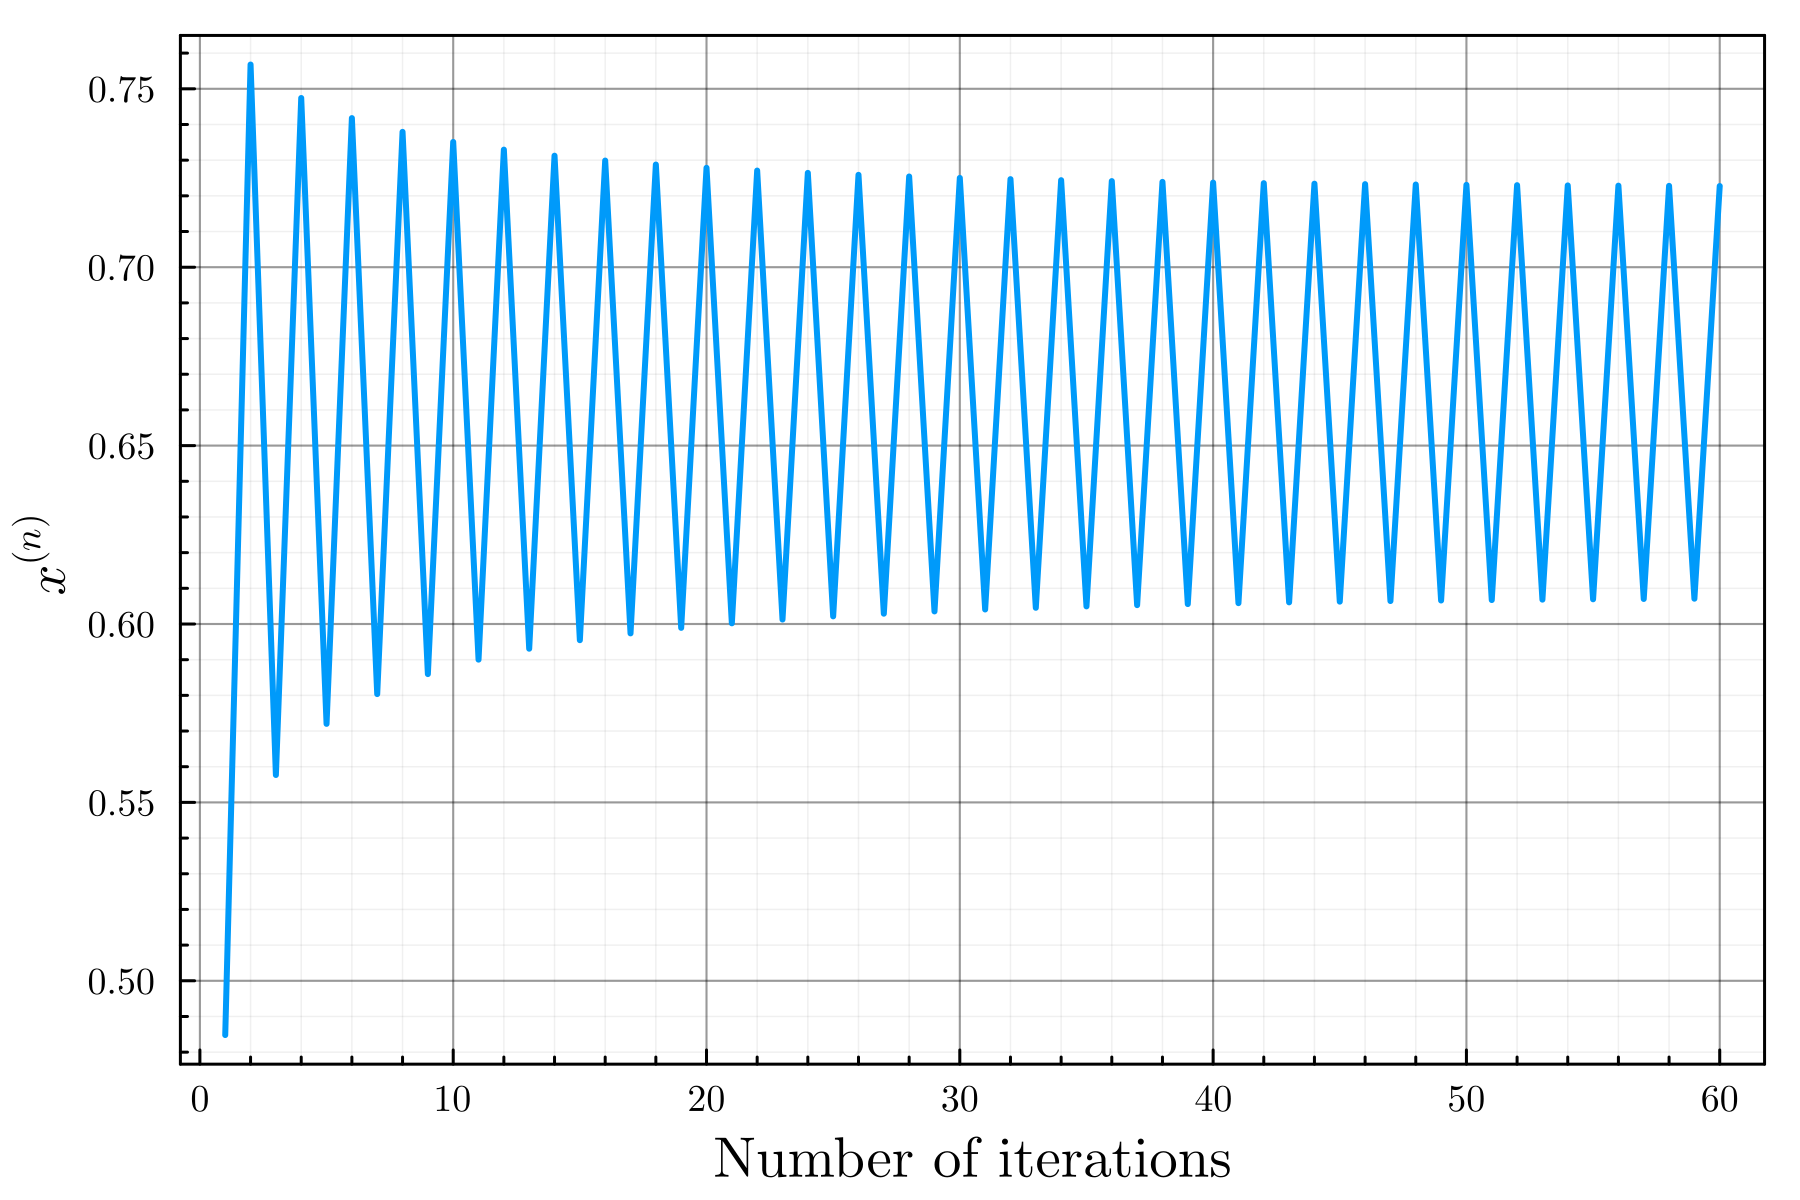
\includegraphics[width=\textwidth]{ch5/convergence_2cycle.png}
        \caption{2-cycle: $r = 3.03$}
    \end{subfigure}
    \hspace{1em}  %\hfill
    \begin{subfigure}[b]{0.45\textwidth}
        \centering
        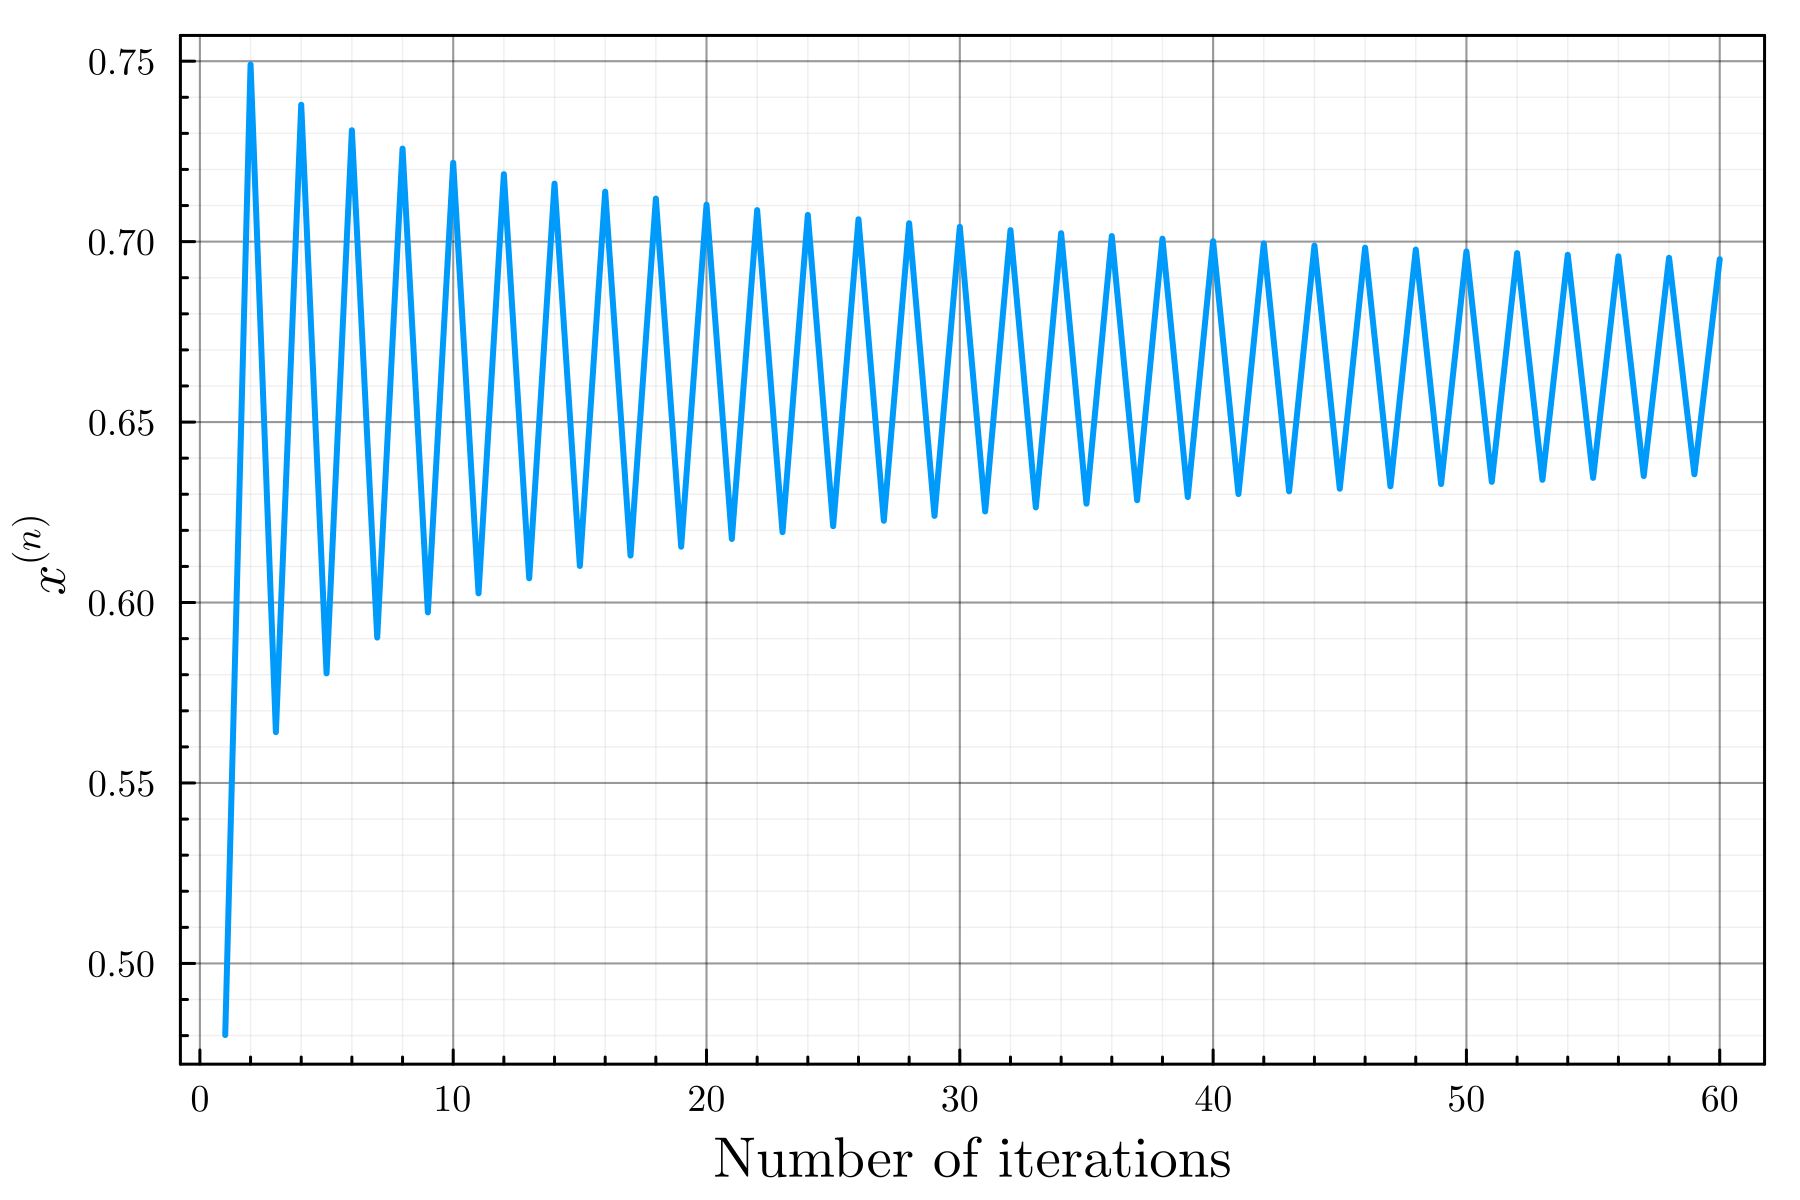
\includegraphics[width=\textwidth]{ch5/convergence_sublinear.png}
        \caption{Sub-linear convergence: $r = 3.001$}
    \end{subfigure}
    \caption{Convergence issues demonstrated using logistic map, $x^{(n+1)} = rx^{(n)}(1 - x^{(n)})$}
    \label{}
\end{figure}
%%% FIG %%%
\FloatBarrier \!\!\!\!\!\!\!\!\!\!\!

\subsection{No convergence}
This generally manifests in the form of 2-cycles. 
\begin{align*}
    f(\{\Psi_A, \Psi_B, \rho_A, \rho_B\}) = \{\Psi_A', \Psi_B', \rho_A', \rho_B'\}\\
    f(\{\Psi_A', \Psi_B', \rho_A', \rho_B'\}) = \{\Psi_A, \Psi_B, \rho_A, \rho_B\}    
\end{align*}

Every 2-cycle encountered also seems to have a pattern that can be exploited to guess the actual fixed point. For example:
\begin{align*}
    &\textbf{2-cycle: }(\Psi_A, \Psi_B, \rho_1, \rho_2) \rightarrow (\Psi_A, \Psi_B, \rho_2, \rho_1)\\
    &\textbf{Fixed point: } (\Psi_A, \Psi_B, (\rho_1 + \rho_2)/2, (\rho_1 + \rho_2)/2)        
\end{align*}

Several patterns like this can emerge, and one solution is to hard-code the guesses for fixed points for each case. This is unfortunately not scalable to arbitrary lattice geometries and parameter regimes. This problem arises from the strong dependancy on the initial guess for the self-consistency loop, and can be remedied by taking several initial guesses till one of them converges.

\subsection{Sub-linear convergence}
This manifests in a form that is decievingly similar to a 2-cycle.
$$f(\{\Psi_A, \Psi_B, \rho_A, \rho_B\}) \approx \{\Psi_A', \Psi_B', \rho_A', \rho_B'\}$$
$$f(\{\Psi_A', \Psi_B', \rho_A', \rho_B'\}) \approx \{\Psi_A, \Psi_B, \rho_A, \rho_B\}$$
The convergence happens at a very slow rate, especially close to the phase boundaries as seen in Fig. \ref{fig:converge_boundary}. This can be handled by utilizing more sophisticated techniques to locate the fixed point such as Nesterov's acceleration. 

%%% FIG %%%
\begin{figure}[!htb]
    \centering
    \begin{subfigure}[b]{0.45\textwidth}  %keep total sum <1 to show in same line
        \centering
        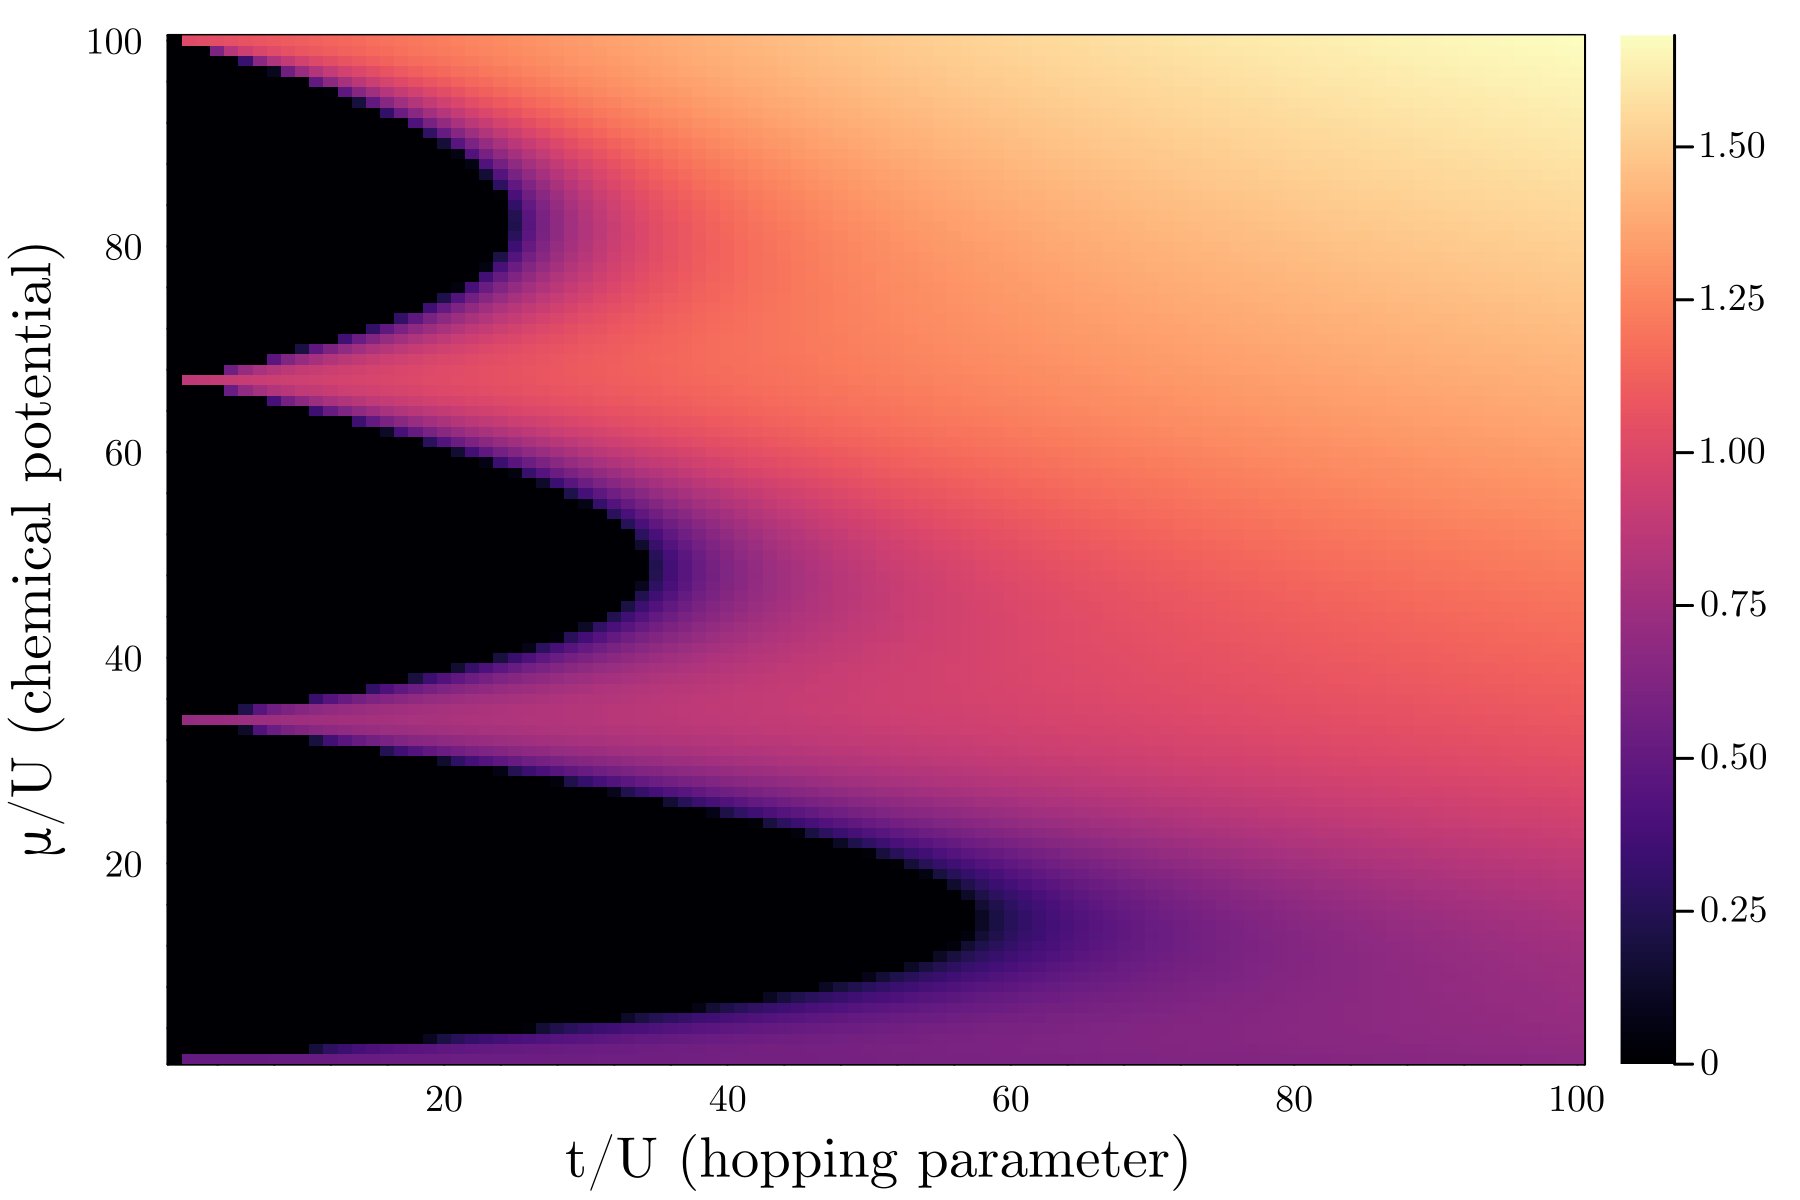
\includegraphics[width=\textwidth]{ch5/bhm_phasediagram.png}
        \caption{Order parameter}
    \end{subfigure}
    \hspace{1em}  %\hfill
    \begin{subfigure}[b]{0.45\textwidth}
        \centering
        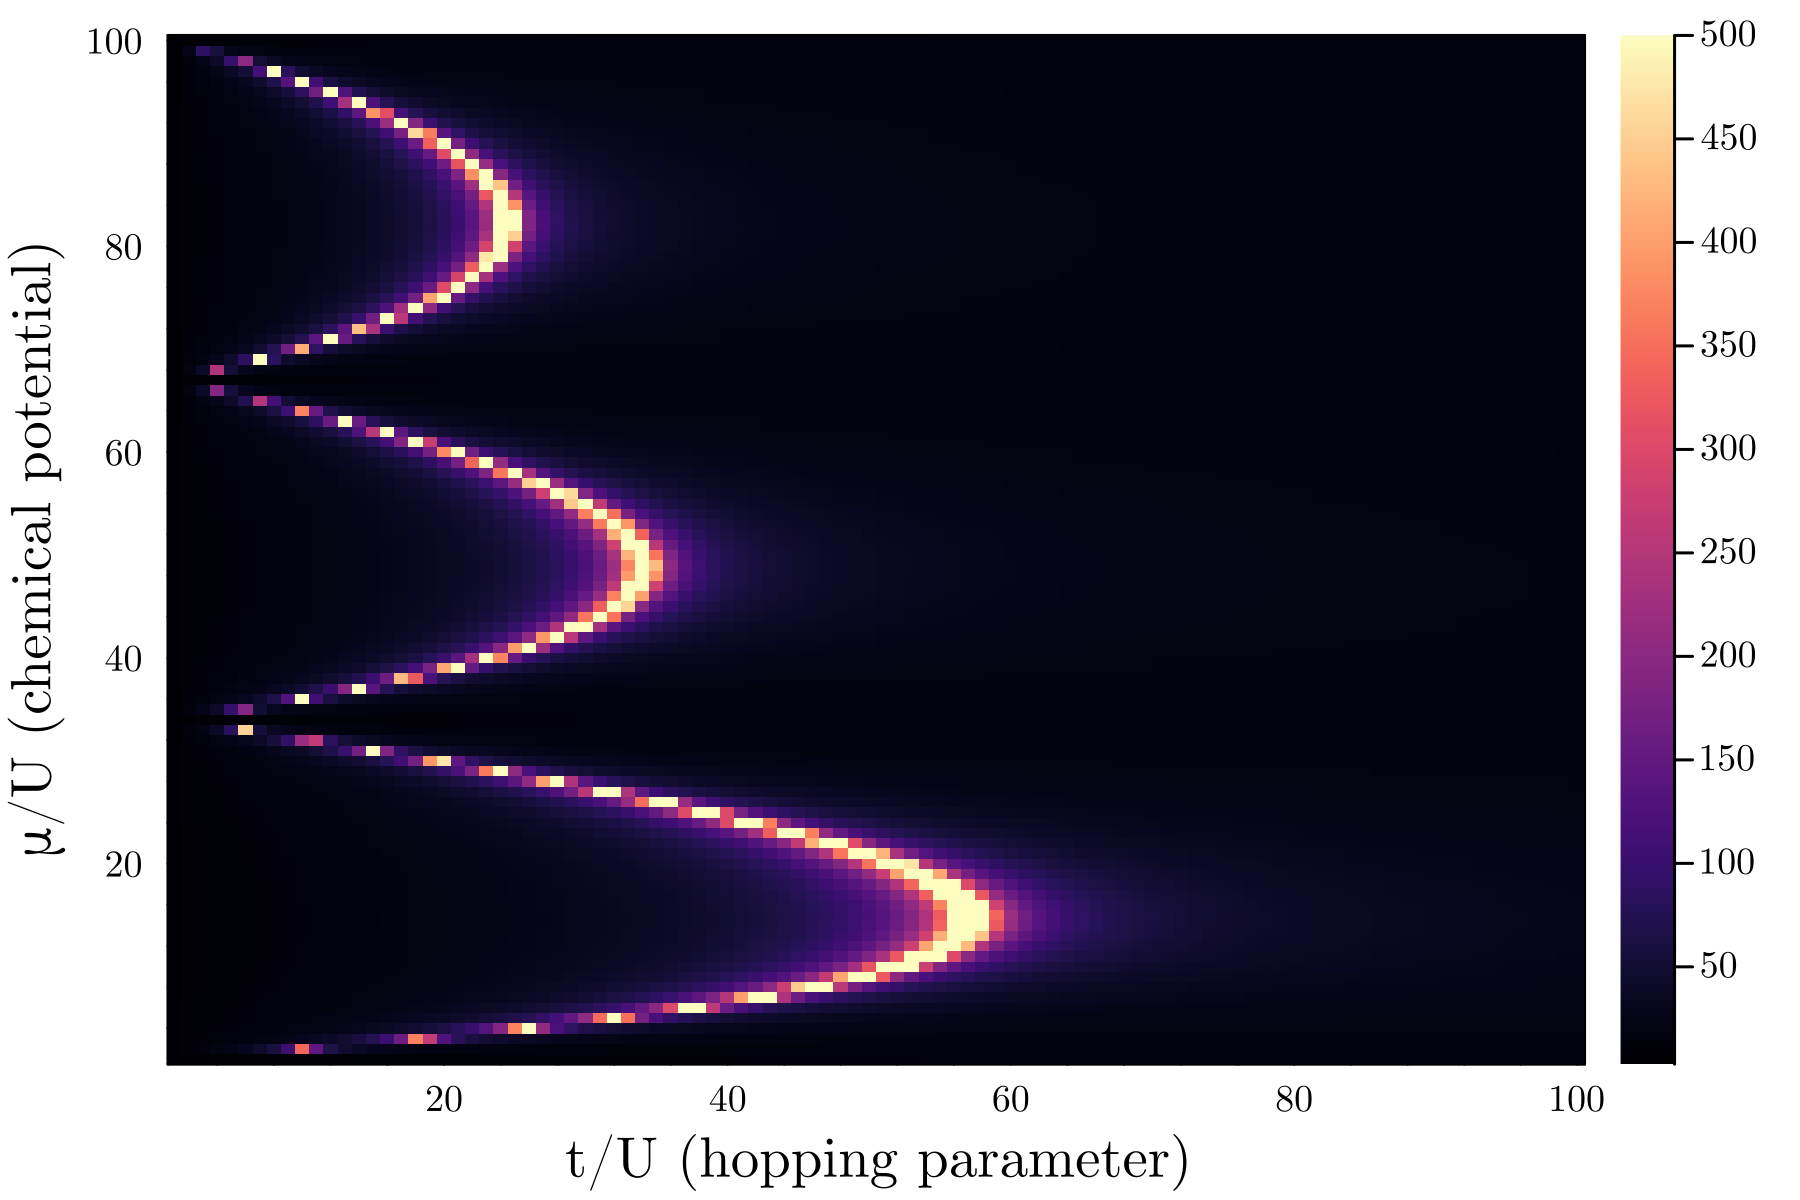
\includegraphics[width=\textwidth]{ch5/bhm_converge.png}
        \caption{Number of iterations}
    \end{subfigure}
    \caption{Nature of convergence near phase boundaries in the BHM}
    \label{fig:converge_boundary}
\end{figure}
%%% FIG %%%
\FloatBarrier \!\!\!\!\!\!\!\!\!\!\!

\subsection{Local minima}
Finally, we come to the important point that there may be several stable fixed points for the same system. By nature of the formulation of the mean-field technique, the true solution is the one with the lowest ground state energy. As a result, we are forced to perform self-consistency starting with a variety of initial guesses to avoid falling into local minima. There does not seem to be a simple way to sample the parameter space in an efficient manner to generate initial guesses. So, an arbitrarily chosen uniform grid was utilized for the results presented in this thesis, but this solution is hardly satisfactory.